% Created 2022-01-20 Thu 11:59
% Intended LaTeX compiler: pdflatex
\documentclass[11pt]{article}
\usepackage[utf8]{inputenc}
\usepackage[T1]{fontenc}
\usepackage{graphicx}
\usepackage{longtable}
\usepackage{wrapfig}
\usepackage{rotating}
\usepackage[normalem]{ulem}
\usepackage{amsmath}
\usepackage{amssymb}
\usepackage{capt-of}
\usepackage{hyperref}
\usepackage{color}
\usepackage{listings}
\usepackage{color}
\usepackage{listings}
\author{Maikol Solís}
\date{2022-01-20}
\title{Emacs workshop 2022: Day 2}
\hypersetup{
 pdfauthor={Maikol Solís},
 pdftitle={Emacs workshop 2022: Day 2},
 pdfkeywords={},
 pdfsubject={},
 pdfcreator={Emacs 27.2 (Org mode 9.6)}, 
 pdflang={English}}
\usepackage{biblatex}

\begin{document}


\section{\texttt{org-mode} introduction}
\label{sec:org42009e8}

\subsection{What is \texttt{org-mode}?}
\label{sec:org0344811}


[[file:org_flow.png]]

\section{Why \texttt{org-mode} and not Markdown?}
\label{sec:orgfef2989}

First Markdown is just a name for many ``flavours''
\begin{itemize}
\item the original implementation (2004)
\item Markdown Extra
\item MultiMarkdown
\item GitHub Flavored Markdown
\item CommonMark which tries to standardize the Markdown standard (again)
\end{itemize}

In general there is no consistency. Some examples:

\begin{itemize}
\item Headings:
\end{itemize}

\begin{verbatim}
 Prefix headings:

 # Heading 1
 ## Heading 2
 ### Heading 3

 Pre- and postfix headings:

 = Heading 1 =
 == Heading 2 ==
 === Heading 3 ===

 Underlined headings:

 Heading 1
 =========

 Heading 2
 ~~~~~~~~~

 Heading 3
 *********
\end{verbatim}

\begin{itemize}
\item Lists:
\end{itemize}

\begin{verbatim}
this

* item 1
* item 2
* item 3

is the same as

- item 1
- item 2
- item 3
\end{verbatim}

A good article about it: \url{https://karl-voit.at/2017/09/23/orgmode-as-markup-only/}


\texttt{Org-mode} is a unified markup language, capable of formating text, run code and export it to multiple formats.
\begin{verbatim}
      |--Code--|             |--Raw Code--> Computer
Ideas-|        |-->Org Mode--|
      |--Text--|             |--Document--> People
\end{verbatim}


\section{Preparation}
\label{sec:orga007264}
\begin{enumerate}
\item Enable export in background
\end{enumerate}
\begin{verbatim}
(setq org-export-in-background t)
\end{verbatim}

\begin{enumerate}
\item Enable pdf module (optional)
\item Use this command \texttt{SPC m e l p}.
\end{enumerate}


\section{Exercises}
\label{sec:org6d98b70}

\subsection{Documentation}
\label{sec:org13c4363}

\url{https://orgmode.org/worg/dev/org-syntax-edited.html}

\subsection{Org-mode syntax}
\label{sec:org48e5c32}

Type of emphasis:

\textbf{bold}
\emph{emphasis}
\texttt{monospace}
\uline{underline}
\texttt{verbatim}
\sout{striketrough}
\(\alpha + \beta\)


\subsection{Headings}
\label{sec:org69b5823}
\begin{itemize}
\item Use levels and stars
\item TODO states
\end{itemize}

\section{{\bfseries\sffamily DONE} Llevar a pasear el perro}
\label{sec:org21a71d1}
\subsection{{\bfseries\sffamily DONE} Nivel 2}
\label{sec:org93bb9aa}
\begin{enumerate}
\item {\bfseries\sffamily DONE} Nivel 3
\label{sec:org03eecde}
\begin{enumerate}
\item {\bfseries\sffamily DONE} Subir el cerro chirripó
\label{sec:org9c8f37d}

\begin{verbatim}
(setq org-todo-keywords
      '((sequence "TODO" "NEXT" "WAIT" "|" "DONE" "CANCELED")))
\end{verbatim}
\end{enumerate}
\end{enumerate}

\subsection{Date and times}
\label{sec:org80e087b}
\begin{itemize}
\item \texttt{SPC m d}
\item Active
\item Inactive
\item Deadline
\item Scheduled
\end{itemize}

\textit{<2022-01-20 Thu 12:00>}
\textit{[2022-01-20 Thu 13:00]}

\subsection{Tareas para el 29 de enero}
\label{sec:orgb809db7}
\begin{enumerate}
\item Tarea 1
\label{sec:orgbb36087}
\item Tarea 2
\label{sec:org9eaf0f5}
\end{enumerate}

\subsection{Priorities}
\label{sec:org73a5842}
\begin{itemize}
\item \texttt{SPC m p}
\item A, B, C
\end{itemize}

\begin{enumerate}
\item Tarea muy importante
\label{sec:orga2d22d3}
\item Tarea mas o menos importante
\label{sec:orga17a4e6}
\item Tarea no importante
\label{sec:orgeb08ba5}
\end{enumerate}

\subsection{Tags}
\label{sec:orgd89e3c3}
\begin{itemize}
\item C-c C-c
\item SPC m q
\end{itemize}

\begin{enumerate}
\item Mi etiquetas\hfill{}\textsc{curso}
\label{sec:org6d45981}
\item Otra etiqueta\hfill{}\textsc{trabajo}
\label{sec:org0d34008}
\end{enumerate}

\subsection{Statistical cookies}
\label{sec:orgaad1395}
\begin{itemize}
\item \texttt{[/]} \texttt{[\%]}
\end{itemize}
\begin{enumerate}
\item\relax [3/3] Projecto
\label{sec:orgc348a21}
\begin{enumerate}
\item {\bfseries\sffamily DONE} Tarea 1
\label{sec:orga4356ee}
\item {\bfseries\sffamily DONE} Tarea 2
\label{sec:orgc6a9eb9}
\item {\bfseries\sffamily DONE} Tarea 3
\label{sec:orgd8e179c}
\end{enumerate}

\item\relax [100\%] Projecto
\label{sec:org753cc91}
\begin{enumerate}
\item {\bfseries\sffamily DONE} Tarea 1
\label{sec:orgdc80b14}
\item {\bfseries\sffamily DONE} Tarea 2
\label{sec:org6315808}
\item {\bfseries\sffamily DONE} Tarea 3
\label{sec:org33e8baf}
\end{enumerate}
\end{enumerate}

\subsection{Plain lists}
\label{sec:org326c330}
\begin{itemize}
\item bullets
\item checkbox
\item statistical cookies
\item start in any number

\item parent item
\begin{itemize}
\item[{$\boxtimes$}] item 1
\item[{$\square$}] item 2
\item[{$\square$}] item 3
\end{itemize}
\end{itemize}

\subsection{CLock in \& Clock out}
\label{sec:org322e17c}
\begin{itemize}
\item SPC m c i
\item SPC m c o
\item org-pomodoro => SPC t t
\end{itemize}


\subsection{Tables}
\label{sec:org4d9afa2}
\begin{itemize}
\item |Name|Phone|Age|
\item |-
\end{itemize}

\begin{center}
\begin{tabular}{lrr}
Name & Phone & Age\\
\hline
Maria & 123 & 25\\
Filomeno & 453 & 30\\
\end{tabular}
\end{center}



\begin{center}
\begin{tabular}{r|rrr|rr|}
N & N\textsuperscript{2} & N\textsuperscript{3} & N\textsuperscript{4} & sqrt(N) & sqrt[4](N)\\
\hline
1 & 1 & 1 & 1 & 1 & 1\\
2 & 4 & 8 & 16 & 1.4142136 & 1.1892071\\
3 & 9 & 27 & 81 & 1.7320508 & 1.3160740\\
\hline
\end{tabular}
\end{center}


\subsection{Links}
\label{sec:orgb520f49}

\begin{center}
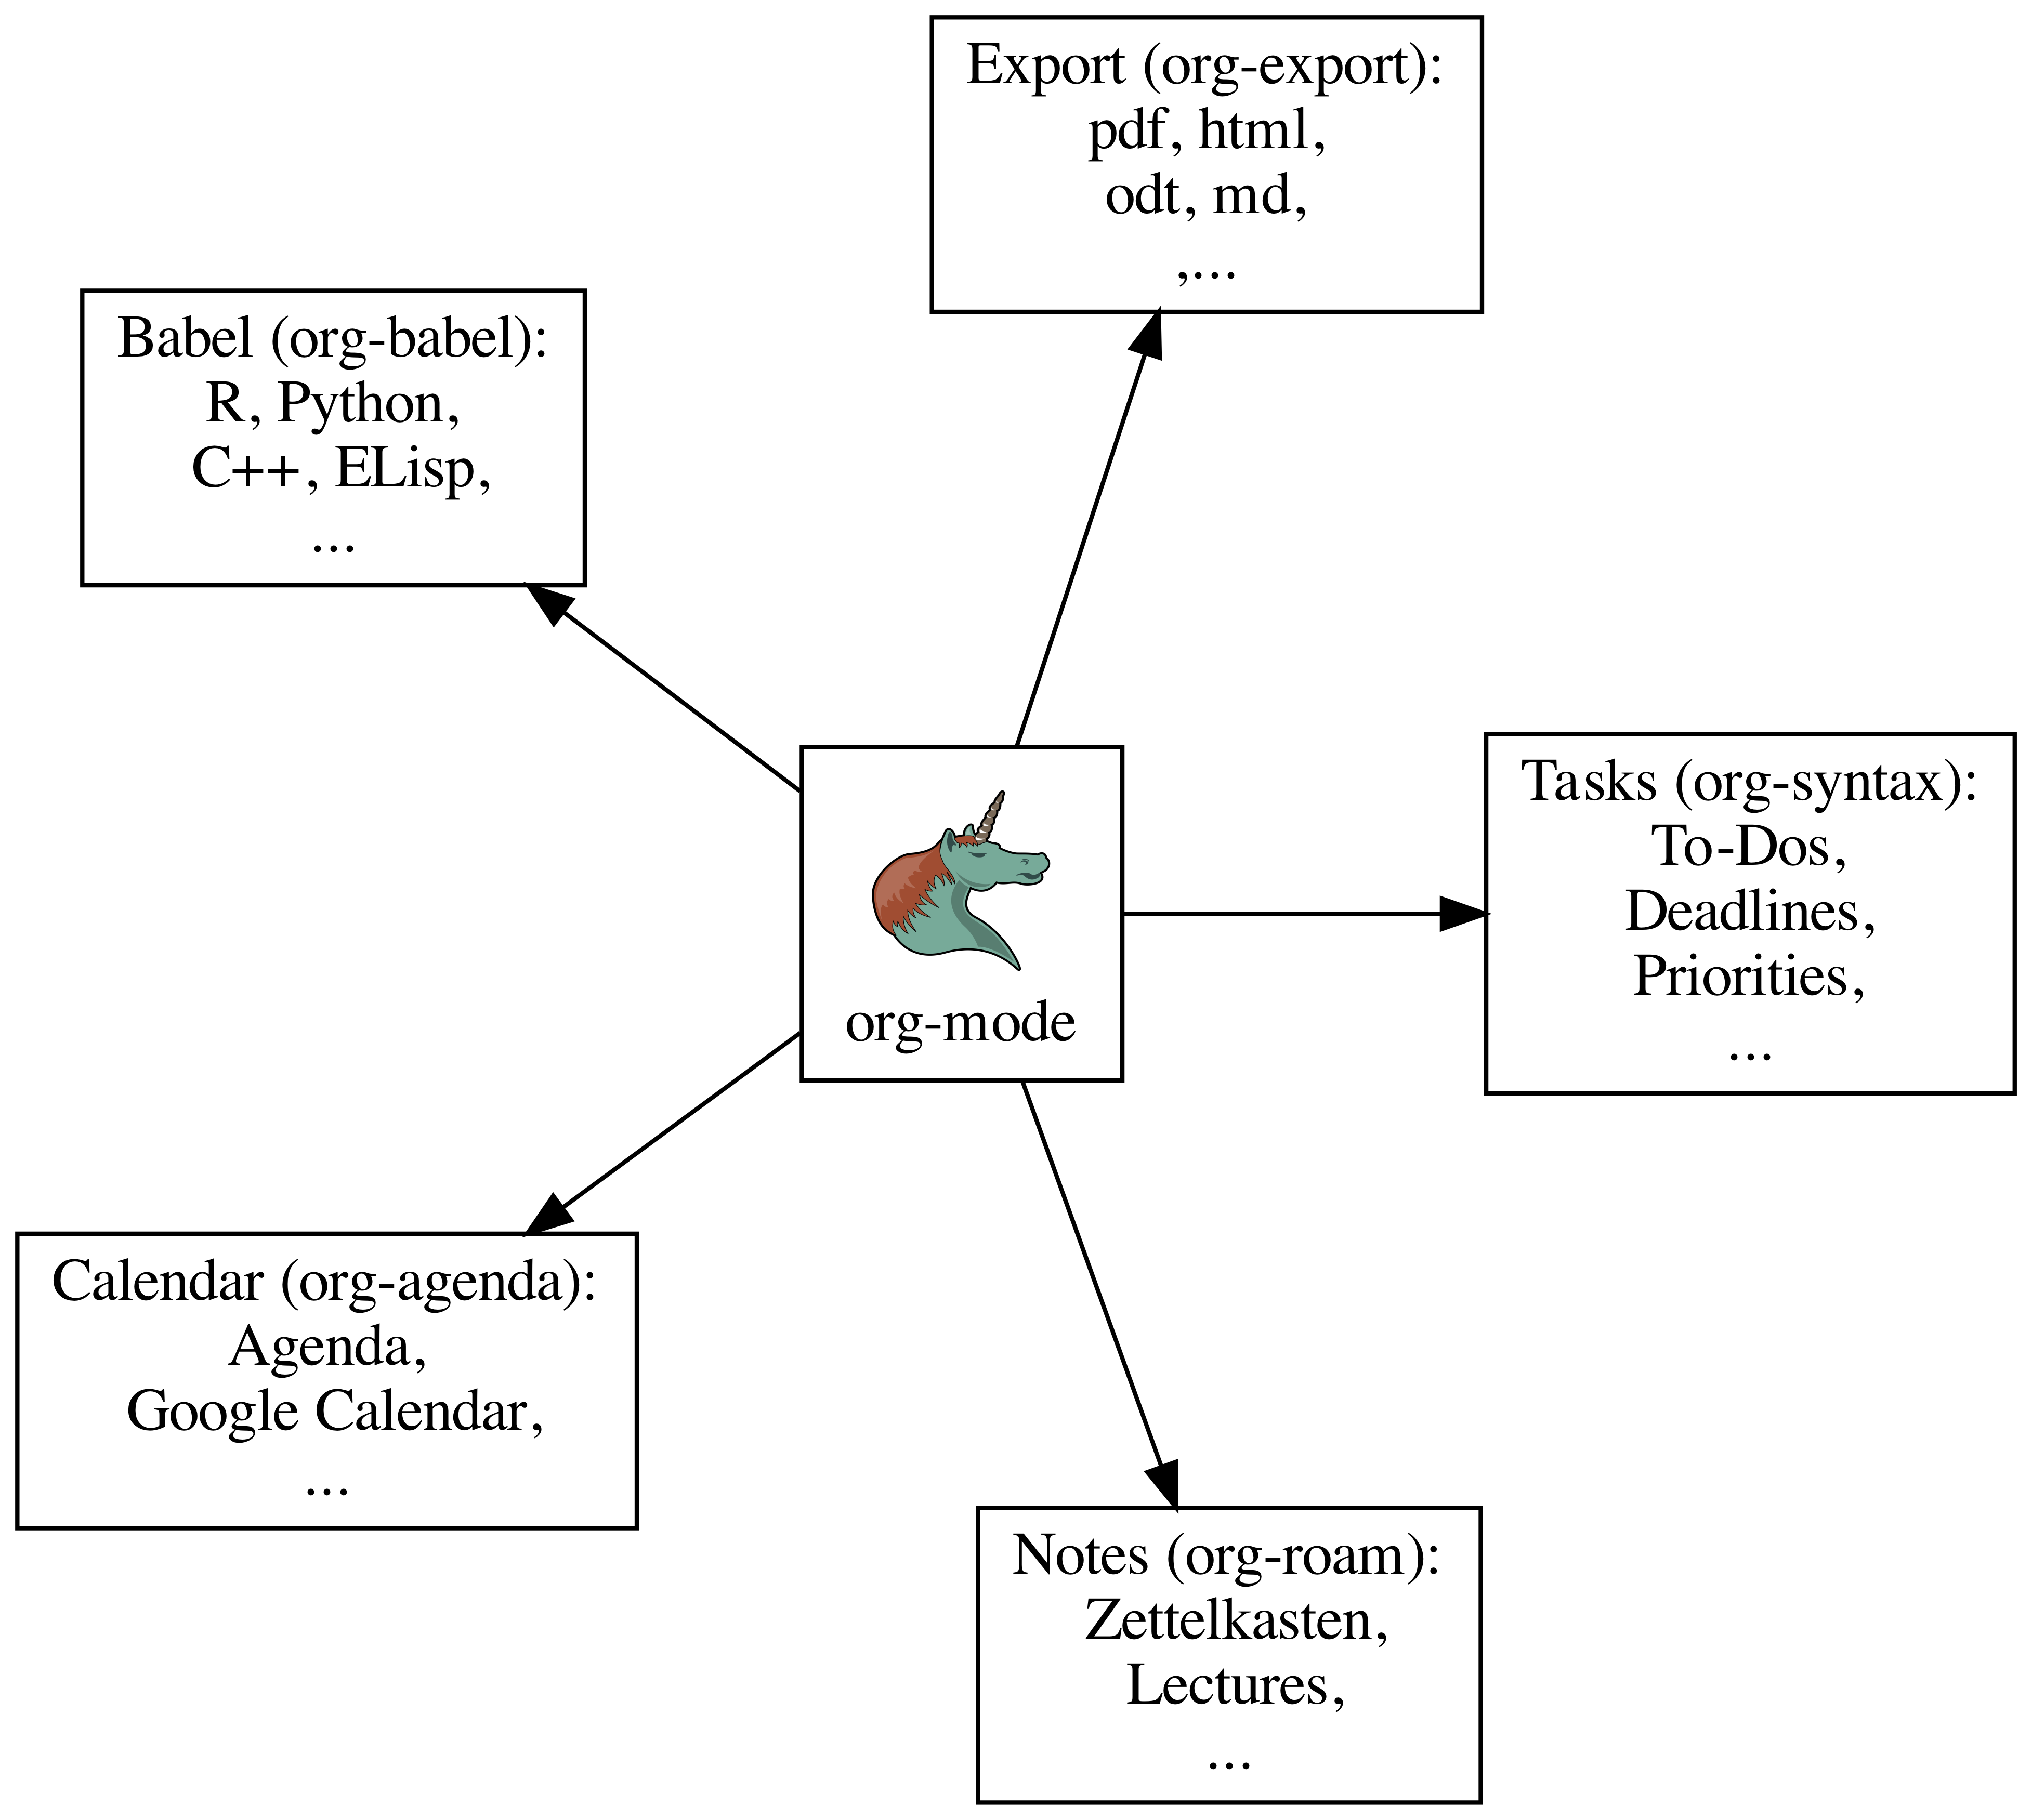
\includegraphics[width=.9\linewidth]{org_flow.png}
\end{center}

\url{../Day\_2}

\url{http://www.google.com}

Aquí está el link de \href{http://www.google.com}{Google}


\subsection{Captions}
\label{sec:orgc29eb25}

\begin{figure}[htbp]
\centering

\includegraphics[width=.9\linewidth]{org_logo.png}
\caption{Org logo}
\end{figure}



\subsection{Labels}
\label{sec:orgdd9d3c0}

\begin{figure}[htbp]
\centering

\includegraphics[width=.9\linewidth]{org_logo.png}
\caption{\label{figura_a_org}Other org logo}
\end{figure}

This is a link to \ref{figura_a_org}


\begin{enumerate}
\item one item
\item \label{target}another item
\end{enumerate}
Here we refer to item \ref{target}.




\subsection{Captures and Templates}
\label{sec:orgd9206aa}


org-mode manual: \url{https://orgmode.org/manual/Capture-templates.html}

\subsection{Agenda views}
\label{sec:org432e55b}


\url{https://orgmode.org/manual/Custom-Agenda-Views.html}
\end{document}